\documentclass[11pt,a4paper]{report}
\usepackage[textwidth=37em,vmargin=30mm]{geometry}
\usepackage{calc,xunicode,amsmath,amssymb,paralist,enumitem,tabu,booktabs,datetime2,xeCJK,xeCJKfntef,listings}
\usepackage{tocloft,fancyhdr,tcolorbox,xcolor,graphicx,eso-pic,xltxtra,xelatexemoji}

\newcommand{\envyear}[0]{2025}
\newcommand{\envdatestr}[0]{2025-02-06}
\newcommand{\envfinaldir}[0]{webdb/2025/20250206/final}

\usepackage[hidelinks]{hyperref}
\hypersetup{
    colorlinks=false,
    pdfpagemode=FullScreen,
    pdftitle={Web Digest - \envdatestr}
}

\setlength{\cftbeforechapskip}{10pt}
\renewcommand{\cftchapfont}{\rmfamily\bfseries\large\raggedright}
\setlength{\cftbeforesecskip}{2pt}
\renewcommand{\cftsecfont}{\sffamily\small\raggedright}

\setdefaultleftmargin{2em}{2em}{1em}{1em}{1em}{1em}

\usepackage{xeCJK,xeCJKfntef}
\xeCJKsetup{PunctStyle=plain,RubberPunctSkip=false,CJKglue=\strut\hskip 0pt plus 0.1em minus 0.05em,CJKecglue=\strut\hskip 0.22em plus 0.2em}
\XeTeXlinebreaklocale "zh"
\XeTeXlinebreakskip = 0pt


\setmainfont{Brygada 1918}
\setromanfont{Brygada 1918}
\setsansfont{IBM Plex Sans}
\setmonofont{JetBrains Mono NL}
\setCJKmainfont{Noto Serif CJK SC}
\setCJKromanfont{Noto Serif CJK SC}
\setCJKsansfont{Noto Sans CJK SC}
\setCJKmonofont{Noto Sans CJK SC}

\setlength{\parindent}{0pt}
\setlength{\parskip}{8pt}
\linespread{1.15}

\lstset{
	basicstyle=\ttfamily\footnotesize,
	numbersep=5pt,
	backgroundcolor=\color{black!5},
	showspaces=false,
	showstringspaces=false,
	showtabs=false,
	tabsize=2,
	captionpos=b,
	breaklines=true,
	breakatwhitespace=true,
	breakautoindent=true,
	linewidth=\textwidth
}






\newcommand{\coverpic}[2]{
    % argv: itemurl, authorname
    Cover photo by #2~~(\href{#1}{#1})
}
\newcommand{\makeheader}[0]{
    \begin{titlepage}
        % \newgeometry{hmargin=15mm,tmargin=21mm,bmargin=12mm}
        \begin{center}
            
            \rmfamily\scshape
            \fontspec{BaskervilleF}
            \fontspec{Old Standard}
            \fontsize{59pt}{70pt}\selectfont
            WEB\hfill DIGEST
            
            \vfill
            % \vskip 30pt
            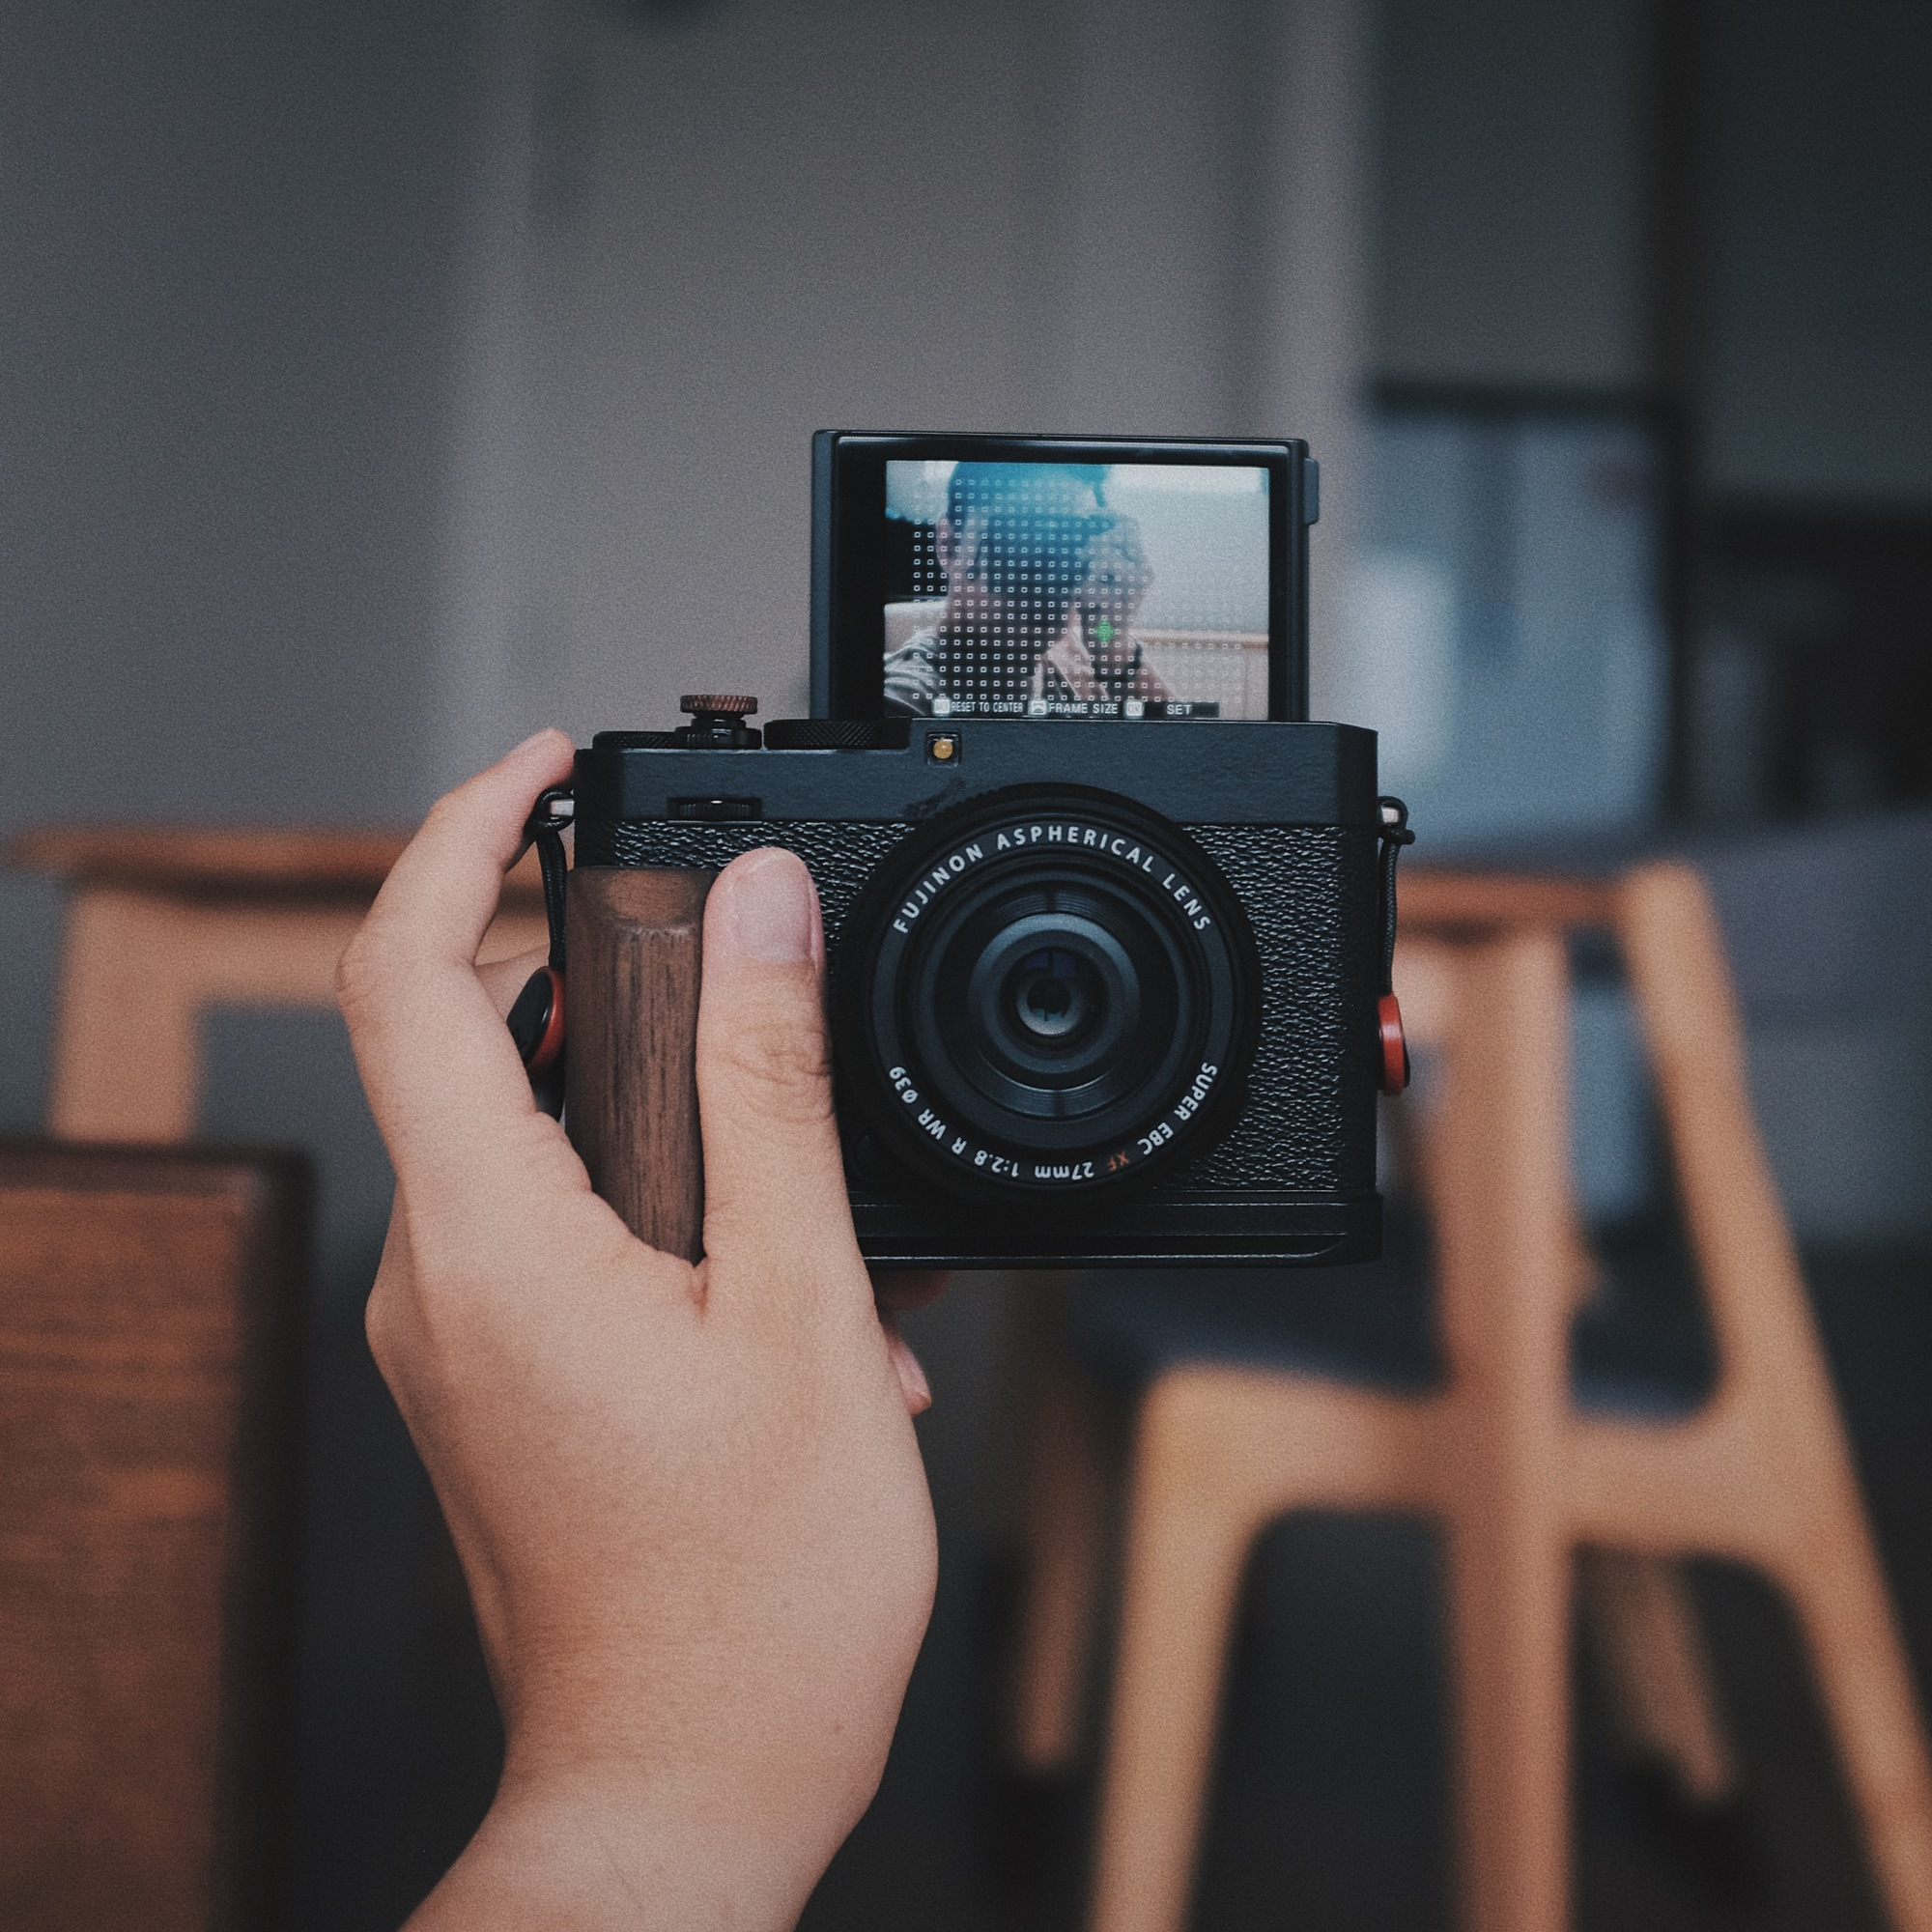
\includegraphics[width=\linewidth]{\envfinaldir/coverpic-prod.jpg}\par
            % \vskip 30pt
            \vfill

            \normalsize\rmfamily\scshape
            \copyright{} The Web Digest Project \hfill\large \envdatestr
        \end{center}
    \end{titlepage}
    % \restoregeometry
}
\newcommand{\simplehref}[1]{%
    \textcolor{blue!80!green}{\href{#1}{#1}}%
}
\renewcommand{\contentsname}{\center\Huge\sffamily\bfseries Contents\par\vskip 20pt}
\newcounter{ipartcounter}
\setcounter{ipartcounter}{0}
\newcommand{\ipart}[1]{
    % \vskip 20pt
    \clearpage
    \stepcounter{ipartcounter}
    \phantomsection
    \addcontentsline{toc}{chapter}{#1}
    % \begin{center}
    %     \Huge
    %     \sffamily\bfseries
    %     #1
    % \end{center}
    % \vskip 20pt plus 7pt
}
\newcounter{ichaptercounter}
\setcounter{ichaptercounter}{0}
\newcommand{\ichapter}[1]{
    % \vskip 20pt
    \clearpage
    \stepcounter{ichaptercounter}
    \phantomsection
    \addcontentsline{toc}{section}{\numberline{\arabic{ichaptercounter}}#1}
    \begin{center}
        \Huge
        \sffamily\bfseries
        #1
    \end{center}
    \vskip 20pt plus 7pt
}
\newcommand{\entrytitlefont}[1]{\subsection*{\raggedright\Large\sffamily\bfseries#1}}
\newcommand{\entryitemGeneric}[2]{
    % argv: title, url
    \parbox{\linewidth}{
        \entrytitlefont{#1}\par\vskip 5pt
        \footnotesize\ttfamily\mdseries
        \simplehref{#2}
    }\vskip 11pt plus 11pt minus 1pt
}
\newcommand{\entryitemGithub}[3]{
    % argv: title, url, desc
    \parbox{\linewidth}{
        \entrytitlefont{#1}\par\vskip 5pt
        \footnotesize\ttfamily\mdseries
        \simplehref{#2}\par\vskip 5pt
        \small\rmfamily\mdseries#3
    }\vskip 11pt plus 11pt minus 1pt
}
\newcommand{\entryitemAp}[3]{
    % argv: title, url, desc
    \parbox{\linewidth}{
        \entrytitlefont{#1}\par\vskip 5pt
        \footnotesize\ttfamily\mdseries
        \simplehref{#2}\par\vskip 5pt
        \small\rmfamily\mdseries#3
    }\vskip 11pt plus 11pt minus 1pt
}
\newcommand{\entryitemHackernews}[3]{
    % argv: title, hnurl, rawurl
    % \parbox{\linewidth}{
    %     \entrytitlefont{#1}\par\vskip 5pt
    %     \footnotesize\ttfamily\mdseries
    %     \simplehref{#3}\par
    %     \textcolor{black!50}{\href{#2}{#2}}
    % }\vskip 11pt plus 11pt minus 1pt
    \begin{minipage}{\linewidth}
            \entrytitlefont{#1}\par\vskip 5pt
            \footnotesize\ttfamily\mdseries
            \simplehref{#3}\par
            \textcolor{black!50}{\href{#2}{#2}}
    \end{minipage}\par\vskip 11pt plus 11pt minus 1pt
}







\begin{document}

\makeheader

\tableofcontents\clearpage




\ipart{Developers}
\ichapter{Hacker News}
\entryitemTwoLinks{Tell HN: Cloudflare is blocking Pale Moon and other non-mainstream browsers}{https://news.ycombinator.com/item?id=42953508}{https://news.ycombinator.com/item?id=42953508}

\entryitemTwoLinks{Zig Guide}{https://news.ycombinator.com/item?id=42953206}{https://zig.guide/}

\entryitemTwoLinks{Andrej Karpathy: Deep Dive into LLMs Like ChatGPT [video]}{https://news.ycombinator.com/item?id=42952960}{https://www.youtube.com/watch?v=7xTGNNLPyMI}

\entryitemTwoLinks{Ingesting PDFs and why Gemini 2.0 changes everything}{https://news.ycombinator.com/item?id=42952605}{https://www.sergey.fyi/articles/gemini-flash-2}

\entryitemTwoLinks{Tesla sales plummet in the UK, France, and Germany}{https://news.ycombinator.com/item?id=42952088}{https://arstechnica.com/cars/2025/02/tesla-sales-plummet-in-the-uk-france-and-germany/}

\entryitemTwoLinks{DOGE employees ordered to stop using Slack}{https://news.ycombinator.com/item?id=42951458}{https://www.404media.co/doge-employees-ordered-to-stop-using-slack-while-agency-transitions-to-a-records-system-not-subject-to-foia/}

\entryitemTwoLinks{Eggs US – Price – Chart}{https://news.ycombinator.com/item?id=42950929}{https://tradingeconomics.com/commodity/eggs-us}

\entryitemTwoLinks{20k federal workers take "buyout" so far, official says}{https://news.ycombinator.com/item?id=42950790}{https://www.axios.com/2025/02/04/trump-buyout-federal-workers-20000}

\entryitemTwoLinks{Gemini 2.0 is now available to everyone}{https://news.ycombinator.com/item?id=42950454}{https://blog.google/technology/google-deepmind/gemini-model-updates-february-2025/}

\entryitemTwoLinks{Servo's progress in 2024}{https://news.ycombinator.com/item?id=42949390}{https://servo.org/blog/2025/01/31/servo-in-2024/}

\entryitemTwoLinks{Avoiding outrage fatigue while staying informed}{https://news.ycombinator.com/item?id=42949277}{https://www.scientificamerican.com/podcast/episode/how-to-avoid-outrage-fatigue-and-tune-in-without-burning-out/}

\entryitemTwoLinks{I'm Done with Ubuntu}{https://news.ycombinator.com/item?id=42949222}{https://ounapuu.ee/posts/2025/02/05/done-with-ubuntu/}

\entryitemTwoLinks{Why is Warner Bros. Discovery putting old movies on YouTube?}{https://news.ycombinator.com/item?id=42949181}{https://tedium.co/2025/02/05/warner-bros-youtube-full-movie-releases/}

\entryitemTwoLinks{F-Droid Awarded Open Technology Fund's FOSS Sustainability Grant}{https://news.ycombinator.com/item?id=42948373}{https://f-droid.org/2025/02/05/f-droid-awarded-otf-grant.html}

\entryitemTwoLinks{Microsoft deletes official Windows 11 CPU/TPM bypass for unsupported PCs}{https://news.ycombinator.com/item?id=42947049}{https://www.neowin.net/news/microsoft-quietly-removes-official-windows-11-cputpm-bypass-for-unsupported-pcs/}

\entryitemTwoLinks{S1: A \$6 R1 competitor?}{https://news.ycombinator.com/item?id=42946854}{https://timkellogg.me/blog/2025/02/03/s1}

\entryitemTwoLinks{Chrome 133 Supports DOM State-Preserving Move with moveBefore()}{https://news.ycombinator.com/item?id=42946718}{https://chromestatus.com/feature/5135990159835136}

\entryitemTwoLinks{Software development topics I've changed my mind on}{https://news.ycombinator.com/item?id=42946281}{https://chriskiehl.com/article/thoughts-after-10-years}

\entryitemTwoLinks{Go Data Structures (2009)}{https://news.ycombinator.com/item?id=42946232}{https://research.swtch.com/godata}

\entryitemTwoLinks{Carl Sagan Predicts the Decline of America (1995)}{https://news.ycombinator.com/item?id=42946046}{https://www.openculture.com/2025/02/carl-sagan-predicts-the-decline-of-america-unable-to-know-whats-true.html}\ichapter{Phoronix}
\entryitemGeneric{\hskip 0pt{}Bisecting The Linux 6.14 Performance Regression With System76 Thelio + AMD Threadripper}{https://www.phoronix.com/news/Linux-6.14-Regression-PM}

\entryitemGeneric{\hskip 0pt{}NVIDIA Engineer Talks Up sched\_ext Linux Scheduler Possibilities At FOSDEM}{https://www.phoronix.com/news/NVIDIA-Talks-Up-Sched-Ext}

\entryitemGeneric{\hskip 0pt{}Linux 6.14 Features Include The AMDXDNA Ryzen AI Driver, NTSYNC, Uncached Buffered I/O \& Much More}{https://www.phoronix.com/review/linux-614-features}

\entryitemGeneric{\hskip 0pt{}AMD Announces Open-Source "Schola" Library For Reinforcement Learning}{https://www.phoronix.com/news/AMD-Schola-Open-Source}

\entryitemGeneric{\hskip 0pt{}AMD Broadcast TLB Invalidation Patches For Linux Updated, Intel RAR Eyed Next}{https://www.phoronix.com/news/AMD-INVLPGB-Linux-v8}

\entryitemGeneric{\hskip 0pt{}Linux Foundation Announces The SEAPATH 1.0 Hypervisor}{https://www.phoronix.com/news/Linux-Foundation-SEAPATH-1.0}

\entryitemGeneric{\hskip 0pt{}Red Hat Developing "F-UKI" As Their Newest Open-Source Project}{https://www.phoronix.com/news/Red-Hat-F-UKI}

\entryitemGeneric{\hskip 0pt{}New Linux Patches Yield Up To 3.3x Faster AES-CTR Performance On AMD Zen 5 CPUs}{https://www.phoronix.com/news/3.3x-AES-CTR-AMD-Zen-5-Patches}

\entryitemGeneric{\hskip 0pt{}cURL 8.12 Released With Its Rust Hyper Backend Removed}{https://www.phoronix.com/news/cURL-8.12-Released}\ichapter{Dribbble}
\entryitemGeneric{\hskip 0pt{}Carbon Solutions B2B Branding Design \& Visual Identity}{https://dribbble.com/shots/25525140-Carbon-Solutions-B2B-Branding-Design-Visual-Identity}

\entryitemGeneric{\hskip 0pt{}Realtree® 30 Years.}{https://dribbble.com/shots/25579343-Realtree-30-Years}

\entryitemGeneric{\hskip 0pt{}VCC Logo Design Vector Sketches}{https://dribbble.com/shots/25577220-VCC-Logo-Design-Vector-Sketches}

\entryitemGeneric{\hskip 0pt{}Brand Family System Loop}{https://dribbble.com/shots/25579103-Brand-Family-System-Loop}

\entryitemGeneric{\hskip 0pt{}Weve Branding}{https://dribbble.com/shots/25579635-Weve-Branding}

\entryitemGeneric{\hskip 0pt{}Chilbot Motion Design}{https://dribbble.com/shots/25578623-Chilbot-Motion-Design}

\entryitemGeneric{\hskip 0pt{}S}{https://dribbble.com/shots/25571540-S}

\entryitemGeneric{\hskip 0pt{}Logo and Branding for VCC}{https://dribbble.com/shots/25571598-Logo-and-Branding-for-VCC}

\entryitemGeneric{\hskip 0pt{}Fly Fry}{https://dribbble.com/shots/25573635-Fly-Fry}

\entryitemGeneric{\hskip 0pt{}Axolotl Mascot}{https://dribbble.com/shots/25572670-Axolotl-Mascot}

\entryitemGeneric{\hskip 0pt{}Finance APP UI Design}{https://dribbble.com/shots/25570740-Finance-APP-UI-Design}

\entryitemGeneric{\hskip 0pt{}Cloud Animation Sound Design}{https://dribbble.com/shots/25571319-Cloud-Animation-Sound-Design}

\entryitemGeneric{\hskip 0pt{}TIAA Duotone Icons}{https://dribbble.com/shots/25573874-TIAA-Duotone-Icons}

\entryitemGeneric{\hskip 0pt{}Year of the Snake}{https://dribbble.com/shots/25563617-Year-of-the-Snake}

\entryitemGeneric{\hskip 0pt{}Atlantic Pickleball Club}{https://dribbble.com/shots/25558009-Atlantic-Pickleball-Club}

\entryitemGeneric{\hskip 0pt{}Wizard Logo}{https://dribbble.com/shots/25559490-Wizard-Logo}

\entryitemGeneric{\hskip 0pt{}Stellar}{https://dribbble.com/shots/25559656-Stellar}

\entryitemGeneric{\hskip 0pt{}VCC Final Logo Animation}{https://dribbble.com/shots/25557794-VCC-Final-Logo-Animation}

\entryitemGeneric{\hskip 0pt{}Saturday Quiz Time Icons}{https://dribbble.com/shots/25561868-Saturday-Quiz-Time-Icons}

\entryitemGeneric{\hskip 0pt{}Crypto onboarding illustrations}{https://dribbble.com/shots/25555520-Crypto-onboarding-illustrations}

\entryitemGeneric{\hskip 0pt{}Shuttle Robotics}{https://dribbble.com/shots/25557675-Shuttle-Robotics}

\entryitemGeneric{\hskip 0pt{}Real Estate Web Design}{https://dribbble.com/shots/25551949-Real-Estate-Web-Design}

\entryitemGeneric{\hskip 0pt{}enso homes}{https://dribbble.com/shots/25552493-enso-homes}

\entryitemGeneric{\hskip 0pt{}Novobet Logo Design - Online Casino Gambling / Betting Platform}{https://dribbble.com/shots/25554663-Novobet-Logo-Design-Online-Casino-Gambling-Betting-Platform}


\ipart{Developers~~~~(zh-Hans)}
\ichapter{Solidot}
\entryitemGeneric{\hskip 0pt{}F-Droid 项目获得约 40 万美元拨款}{https://www.solidot.org/story?sid=80479}

\entryitemGeneric{\hskip 0pt{}泰国对妙瓦底等缅甸地区断电断网}{https://www.solidot.org/story?sid=80478}

\entryitemGeneric{\hskip 0pt{}DeepSeek 研究称华为昇腾 910C 推理性能能达到英伟达 H100 的六成}{https://www.solidot.org/story?sid=80477}

\entryitemGeneric{\hskip 0pt{}AI 生成内容进入了公共图书馆}{https://www.solidot.org/story?sid=80476}

\entryitemGeneric{\hskip 0pt{}天文学家在系外行星上发现风速高达 9 公里/秒的超音速气流}{https://www.solidot.org/story?sid=80475}

\entryitemGeneric{\hskip 0pt{}Paragon 证实美国及其盟国是其客户}{https://www.solidot.org/story?sid=80474}

\entryitemGeneric{\hskip 0pt{}美国邮政停收内地和香港的包裹 }{https://www.solidot.org/story?sid=80473}

\entryitemGeneric{\hskip 0pt{}Google 更新 AI 政策移除了不将 AI 用于武器和监视的承诺}{https://www.solidot.org/story?sid=80472}

\entryitemGeneric{\hskip 0pt{}波兰逮捕批准购买间谍软件 Pegasus 的前司法部长}{https://www.solidot.org/story?sid=80471}

\entryitemGeneric{\hskip 0pt{}FSF 将在下月拍卖纪念品}{https://www.solidot.org/story?sid=80470}

\entryitemGeneric{\hskip 0pt{}Framework 推出售价 199 美元的 RISC-V 主板}{https://www.solidot.org/story?sid=80469}

\entryitemGeneric{\hskip 0pt{}工商总局对谷歌发起反垄断调查}{https://www.solidot.org/story?sid=80468}

\entryitemGeneric{\hskip 0pt{}Freedesktop 和 Alpine Linux 寻找新托管商}{https://www.solidot.org/story?sid=80467}

\entryitemGeneric{\hskip 0pt{}天文学家发现一巨型射电星系}{https://www.solidot.org/story?sid=80466}

\entryitemGeneric{\hskip 0pt{}过去四十年海洋表面变暖速度翻了两番}{https://www.solidot.org/story?sid=80465}

\entryitemGeneric{\hskip 0pt{}Ubuntu 的开发讨论平台将从 IRC 迁移到 Matrix}{https://www.solidot.org/story?sid=80464}\ichapter{V2EX}
\entryitemGeneric{\hskip 0pt{}[Linux] 奇怪的 pve 故障}{https://www.v2ex.com/t/1109212}

\entryitemGeneric{\hskip 0pt{}[分享发现] ARK Invest(木头姐)的 2025 BIG IDEAS,欢迎阅读}{https://www.v2ex.com/t/1109211}

\entryitemGeneric{\hskip 0pt{}[分享创造] JSON 格式化网站千千万,为何我又造了一个}{https://www.v2ex.com/t/1109210}

\entryitemGeneric{\hskip 0pt{}[美酒与美食] 红枣泡水,口感真不错,甘甜,顺带小结一下不同花茶、代茶的口感}{https://www.v2ex.com/t/1109209}

\entryitemGeneric{\hskip 0pt{}[职场话题] 想去国外工作,可以有哪些路子?}{https://www.v2ex.com/t/1109208}

\entryitemGeneric{\hskip 0pt{}[程序员] 想问下在腾讯年薪 200 万属于什么段位?比如要管多大的项目或者管多少人?}{https://www.v2ex.com/t/1109206}

\entryitemGeneric{\hskip 0pt{}[问与答] 安卓系统有什么渠道/APP 长期免费看 CBA 篮球}{https://www.v2ex.com/t/1109205}

\entryitemGeneric{\hskip 0pt{}[分享创造] 分享一个独立开发者开发国际化项目提效的思路}{https://www.v2ex.com/t/1109204}

\entryitemGeneric{\hskip 0pt{}[程序员] PPT / 规划 / 总结 / 汇报能力如何提升?}{https://www.v2ex.com/t/1109203}

\entryitemGeneric{\hskip 0pt{}[问与答] 考研考杭州电子科技大学怕考不上,可以考浙工大或者浙理工吗?}{https://www.v2ex.com/t/1109202}

\entryitemGeneric{\hskip 0pt{}[分享创造] 迁移网站到 nextjs 了}{https://www.v2ex.com/t/1109200}

\entryitemGeneric{\hskip 0pt{}[iPhone] iOS 代理工具哪个最省电呢?}{https://www.v2ex.com/t/1109199}

\entryitemGeneric{\hskip 0pt{}[Apple] mac 端的日历同步到 iPhone 端后看不到附件}{https://www.v2ex.com/t/1109198}

\entryitemGeneric{\hskip 0pt{}[宽带症候群] 珍爱生命,远离 qq 音乐}{https://www.v2ex.com/t/1109197}

\entryitemGeneric{\hskip 0pt{}[问与答] 结婚多年后发现,上交工资卡是最愚蠢的行为。}{https://www.v2ex.com/t/1109196}

\entryitemGeneric{\hskip 0pt{}[程序员] 准备 boss 直聘体验下地狱级面试难度纪念 35 岁}{https://www.v2ex.com/t/1109192}

\entryitemGeneric{\hskip 0pt{}[分享发现] WiFi 连接解决方案 - 二维码极速联网}{https://www.v2ex.com/t/1109191}

\entryitemGeneric{\hskip 0pt{}[分享创造] [问与答] 被裁员后,我在考虑做一个 AI 面试助手,有需求吗?}{https://www.v2ex.com/t/1109190}

\entryitemGeneric{\hskip 0pt{}[职场话题] 因项目延期不断焦虑,不安,应该怎么办?}{https://www.v2ex.com/t/1109189}

\entryitemGeneric{\hskip 0pt{}[问与答] 父母都是农民,还没到 60,要补缴养老保险吗?}{https://www.v2ex.com/t/1109188}

\entryitemGeneric{\hskip 0pt{}[投资] iOS 端有推荐的看黄金金价的软件吗?}{https://www.v2ex.com/t/1109185}

\entryitemGeneric{\hskip 0pt{}[iPad] 关于国行 iPad 使用 apple intelligence?}{https://www.v2ex.com/t/1109184}

\entryitemGeneric{\hskip 0pt{}[宽带症候群] 请教关于使用 TR069 连接组网,并实现 Internet 访问的实现}{https://www.v2ex.com/t/1109183}

\entryitemGeneric{\hskip 0pt{}[分享创造] 做了一个 windows 的搜索文件的 app,有没有老哥感兴趣帮忙内测的}{https://www.v2ex.com/t/1109181}

\entryitemGeneric{\hskip 0pt{}[问与答] 2024 年终总结,今年本命年感觉自己变得格外的絮絮叨叨}{https://www.v2ex.com/t/1109180}

\entryitemGeneric{\hskip 0pt{}[问与答] 想问问大家从多少岁就开始不敢轻易裸辞了}{https://www.v2ex.com/t/1109179}

\entryitemGeneric{\hskip 0pt{}[投资] 现在的黄金金价处于高位,为什么还有那么多人购买?}{https://www.v2ex.com/t/1109178}

\entryitemGeneric{\hskip 0pt{}[JetBrains] JetBrains 新退出的 Junie 有用过的吗?}{https://www.v2ex.com/t/1109177}

\entryitemGeneric{\hskip 0pt{}[宽带症候群] 上海联通 9929 到日本 NTT 速度很拉跨}{https://www.v2ex.com/t/1109176}

\entryitemGeneric{\hskip 0pt{}[OpenAI] 128G 内存的 Macbook 能跑动 Deepseek 70b 的模型吗}{https://www.v2ex.com/t/1109174}

\entryitemGeneric{\hskip 0pt{}[生活] 聊一聊患病住院的经历}{https://www.v2ex.com/t/1109171}

\entryitemGeneric{\hskip 0pt{}[职场话题] 0 负债了!纪念一下!}{https://www.v2ex.com/t/1109170}

\entryitemGeneric{\hskip 0pt{}[ WATCH] watch 睡眠闹铃不响,健康数据和三色环数据不能及时同步}{https://www.v2ex.com/t/1109168}

\entryitemGeneric{\hskip 0pt{}[输入法] 微信输入法怎么中英混合输入?}{https://www.v2ex.com/t/1109167}

\entryitemGeneric{\hskip 0pt{}[硬件] 老人家里没 wifi,求推荐老年智能手表或家用监控。}{https://www.v2ex.com/t/1109166}

\entryitemGeneric{\hskip 0pt{}[问与答] Mac 上有没有什么软件可以把刘海两侧的空间上放点小玩意儿利用起来}{https://www.v2ex.com/t/1109165}

\entryitemGeneric{\hskip 0pt{}[杭州] 10 年北漂想入杭有啥建议吗}{https://www.v2ex.com/t/1109164}

\entryitemGeneric{\hskip 0pt{}[宽带症候群] unifiOS 下,如何在 ipv6 的网络设置中引入旁路网关的 ipv6 地址}{https://www.v2ex.com/t/1109163}

\entryitemGeneric{\hskip 0pt{}[生活] 感觉 微信公众号、B 站等也都开始擦边了。这算是劣币驱逐良币么?}{https://www.v2ex.com/t/1109162}

\entryitemGeneric{\hskip 0pt{}[酷工作] [广州-三七互娱-社招]资深 golang 开发工程师、高级 golang 开发工程师、高级运维开发工程师}{https://www.v2ex.com/t/1109161}

\entryitemGeneric{\hskip 0pt{}[奇思妙想] 如果你的微信好友都是 AI 扮演,只有你是真人,好玩还是恐怖?}{https://www.v2ex.com/t/1109160}

\entryitemGeneric{\hskip 0pt{}[OpenAI] AI 解析表格图片总是错乱,有什么好的办法}{https://www.v2ex.com/t/1109158}

\entryitemGeneric{\hskip 0pt{}[Apple] 1k 的全原美版刚过保 se3 64g 值吗?}{https://www.v2ex.com/t/1109157}

\entryitemGeneric{\hskip 0pt{}[宽带症候群] 关于 ss 回家相关问题}{https://www.v2ex.com/t/1109156}

\entryitemGeneric{\hskip 0pt{}[职场话题] 收了 1000 多开工红包,发了 700,图个开心}{https://www.v2ex.com/t/1109155}

\entryitemGeneric{\hskip 0pt{}[推广] 我的网站第一天放谷歌广告,收入 5 美元}{https://www.v2ex.com/t/1109154}

\entryitemGeneric{\hskip 0pt{}[问与答] Swift 操作 plist 文件}{https://www.v2ex.com/t/1109153}

\entryitemGeneric{\hskip 0pt{}[问与答] IT 码农,抬头没脖子怎么办(没下颚线)}{https://www.v2ex.com/t/1109152}

\entryitemGeneric{\hskip 0pt{}[信息安全] LUKS 加密磁盘后的 vps 是不是就彻底安全了,求指教}{https://www.v2ex.com/t/1109151}

\entryitemGeneric{\hskip 0pt{}[宽带症候群] 含 300M+带宽、流量 50G+、月租 40,有没有这样的手机卡?}{https://www.v2ex.com/t/1109150}


\ipart{Generic News}
\ichapter{AP News}
\entryitemWithDescription{\hskip 0pt{}Super Bowl secondary-ticket prices high but much less than last year's game}{https://apnews.com/article/cd6049fcad6400be24a8bde82e20fc37}{}

\entryitemWithDescription{\hskip 0pt{}Ozzy Osbourne to reunite with Black Sabbath bandmates in Birmingham for `greatest' show ever}{https://apnews.com/article/e46239b93d954e5d464d44554d6cff64}{}

\entryitemWithDescription{\hskip 0pt{}AI and scientists unite to decipher old scrolls charred by the Vesuvius volcano}{https://apnews.com/article/22506589e8ad28efc59ce05224bf6657}{}

\entryitemWithDescription{\hskip 0pt{}Scientists solve the mystery of sea turtles' `lost years'}{https://apnews.com/article/f92a0c5447cd710f189e6789bab6c78d}{}

\entryitemWithDescription{\hskip 0pt{}Earthquakes keep rattling Greece's volcanic island of Santorini every few minutes}{https://apnews.com/article/7ffcbc139ad1081acdad181df1ad2952}{}

\entryitemWithDescription{\hskip 0pt{}Box-office smash `Moana 2' drives Disney profit in the first quarter}{https://apnews.com/article/c2128459cbe670c85f2f374669954a99}{}

\entryitemWithDescription{\hskip 0pt{}Making climate-friendly lifestyle choices isn't always easy. India learned the hard way}{https://apnews.com/article/ec1700fb6eea9b730c63b4394b627623}{}

\entryitemWithDescription{\hskip 0pt{}The Aga Khan, spiritual leader of Ismaili Muslims and a philanthropist, dies at 88}{https://apnews.com/article/568f5859ac60d11f2eac2abf793d81f5}{}

\entryitemWithDescription{\hskip 0pt{}Tiger Woods says his mother has died. He called Kultida Woods a `force of nature'}{https://apnews.com/article/90f1b2500db0f45f931c699d193c3482}{}

\entryitemWithDescription{\hskip 0pt{}The colors we see make a difference in the food we eat}{https://apnews.com/article/a7e0ab3cbb08a8e408d1ad9d0da8420c}{}

\entryitemWithDescription{\hskip 0pt{}Decorated pilot Harry Stewart, Jr., one of the last surviving Tuskegee Airmen, dies at 100}{https://apnews.com/article/78fd504895d7af70d4bb1e2243a54ee6}{}

\entryitemWithDescription{\hskip 0pt{}An Arkansas organist is playing 18 hours of Bach this year, one lunch break at a time}{https://apnews.com/article/83ba3ee8d72e2d9cf4a331eaaaaa21b5}{}

\entryitemWithDescription{\hskip 0pt{}Hundreds join an order of naked, armed holy men at Hindu festival}{https://apnews.com/article/dda7ba7c65ccfa7ad530d26a5d6374a3}{}\ichapter{Reuters}
\entryitemWithDescription{\hskip 0pt{}Russian diplomat says US must make first step to improve ties}{https://www.reuters.com/world/russian-diplomat-says-us-must-make-first-step-improve-ties-2025-02-05/}{The United States must make the first move in improving ties with Russia after years of failing to listen to the Kremlin and misguided policies intended to inflict a "strategic defeat" on Moscow, a senior Russian diplomat said on...}

\entryitemWithDescription{\hskip 0pt{}Explainer: What to know about Trump's Gaza Strip proposal}{https://www.reuters.com/world/us/what-know-about-trumps-gaza-strip-proposal-2025-02-05/}{President Donald Trump\textquotesingle s plan for the United States to take over Gaza, permanently displacing Palestinians who live there and creating the "Riviera of the Middle East," has upset Arab nations and Western allies and would...}

\entryitemWithDescription{\hskip 0pt{}Canada says its position on Gaza has not changed, backs two-state solution}{https://www.reuters.com/world/canada-says-its-position-gaza-has-not-changed-backs-two-state-solution-2025-02-05/}{Canada\textquotesingle s longstanding position on Gaza has not changed and it is committed to achieving a two-state solution, Foreign Minister Melanie Joly said in a post on X on...}

\entryitemWithDescription{\hskip 0pt{}US military prepared to look at all options for Gaza, US defense secretary says}{https://www.reuters.com/world/us-military-prepared-look-all-options-gaza-us-defense-secretary-says-2025-02-05/}{U.S. Defense Secretary Pete Hegseth said on Wednesday the Pentagon was prepared to look at all options for Gaza, a day after President Donald Trump said he would like the U.S. to take control of and redevelop the Gaza...}

\entryitemWithDescription{\hskip 0pt{}Immigration raids target alleged Venezuelan gang members in Aurora, Colorado}{https://www.reuters.com/world/americas/immigration-raids-target-alleged-venezuelan-gang-members-aurora-colorado-2025-02-05/}{Officers from several U.S. federal agencies searched for alleged members of Venezuelan street gang Tren de Aragua on Wednesday in Aurora, the Colorado city with a large migrant population where President Donald Trump laid out his...}

\entryitemWithDescription{\hskip 0pt{}Syria's president receives invitation from Macron to visit France in coming weeks, Syrian presidency says}{https://www.reuters.com/world/syrias-president-receives-invitation-macron-visit-france-coming-weeks-syrian-2025-02-05/}{Syria\textquotesingle s President Ahmed al-Sharaa received an invitation from French President Emmanuel Macron to visit France in the coming weeks, the Syrian president\textquotesingle s office said in a statement on...}

\entryitemWithDescription{\hskip 0pt{}Arab American, Muslim leaders decry Trump comments on Gaza}{https://www.reuters.com/world/us/arab-american-muslim-leaders-decry-trump-comments-gaza-2025-02-05/}{U.S. Arab American and Muslim leaders, including some who supported Donald Trump in the 2024 election, criticized the president\textquotesingle s proposal for the U.S. to take over Gaza and resettle Palestinians, but some of them said...}

\entryitemWithDescription{\hskip 0pt{}Lara Trump to host weekend primetime program on Fox News Channel}{https://www.reuters.com/world/us/lara-trump-host-weekend-primetime-program-fox-news-channel-2025-02-05/}{Lara Trump, daughter-in-law of U.S. President Donald Trump, is set to host a new weekend primetime program on Fox News Channel starting the end of this month, the Fox Corp owned news service said on...}

\entryitemWithDescription{\hskip 0pt{}Trump has offered for US to be responsible for reconstruction of Gaza, Rubio says}{https://www.reuters.com/world/trump-has-offered-us-be-responsible-reconstruction-gaza-rubio-says-2025-02-05/}{U.S. President Donald Trump has offered for the United States to be responsible for the reconstruction of Gaza, Secretary of State Marco Rubio said on Wednesday, after the president proposed a U.S. takeover of the...}

\entryitemWithDescription{\hskip 0pt{}Guatemala to accept more US deportation flights after Rubio talks}{https://www.reuters.com/world/americas/guatemala-says-it-will-increase-number-deportation-flights-it-accepts-us-2025-02-05/}{Guatemala will accept 40\% more deportation flights including both Guatemalan deportees and those of other...}

\entryitemWithDescription{\hskip 0pt{}United Nations chief warns Trump against ethnic cleansing in Gaza}{https://www.reuters.com/world/middle-east/un-chief-say-its-essential-ethnic-cleansing-be-avoided-gaza-says-spokesperson-2025-02-05/}{United Nations Secretary-General Antonio Guterres told President Donald Trump on Wednesday to avoid ethnic cleansing in Gaza after the U.S. leader proposed that Palestinians resettle elsewhere and the United States take over the war-torn...}

\entryitemWithDescription{\hskip 0pt{}Judge blocks Sandy Hook families' settlement in Alex Jones' bankruptcy}{https://www.reuters.com/world/us/judge-blocks-sandy-hook-families-settlement-alex-jones-bankruptcy-2025-02-05/}{A U.S. bankruptcy judge on Wednesday blocked a settlement between families who have sued Alex Jones over his false claims about the 2012 Sandy Hook Elementary School mass shooting, saying their attempt to divide the bankrupt conspiracy...}

\entryitemWithDescription{\hskip 0pt{}How Trump's Gaza proposals could violate international law}{https://www.reuters.com/world/middle-east/how-trumps-gaza-proposals-could-violate-international-law-2025-02-05/}{U.S. President Donald Trump said he wants to resettle Palestinians from the Gaza Strip to Egypt and Jordan, demolish remaining buildings to make way for a Riviera-style development project and place the occupied territory under U.S. "...}






\clearpage
\leavevmode\vfill
\footnotesize

Copyright \copyright{} 2023-2025 Neruthes and other contributors.

This document is published with CC BY-NC-ND 4.0 license.

The entries listed in this newsletter may be copyrighted by their respective creators.

This newsletter is generated by the Web Digest project.

The newsletters are also delivered via Telegram channel \CJKunderline{\href{https://t.me/webdigestchannel}{https://t.me/webdigestchannel}}.\\
RSS feed is available at \CJKunderline{\href{https://webdigest.pages.dev/rss.xml}{https://webdigest.pages.dev/rss.xml}}.

This newsletter is available in PDF at
\CJKunderline{\href{https://webdigest.pages.dev/}{https://webdigest.pages.dev/}}.

The source code being used to generate this newsletter is available at\\
\CJKunderline{\href{https://github.com/neruthes/webdigest}{https://github.com/neruthes/webdigest}}.

This newsletter is also available in
\CJKunderline{\href{http://webdigest.pages.dev/readhtml/\envyear/WebDigest-20250206.html}{HTML}} and
\CJKunderline{\href{https://github.com/neruthes/webdigest/blob/master/markdown/\envyear/WebDigest-20250206.md}{Markdown}}.


\coverpic{https://unsplash.com/photos/a-large-white-house-sitting-in-the-middle-of-a-forest-\_K4d19tmLQU}{Adrian Botica}


\end{document}
